\documentclass[11pt]{scrartcl}

\usepackage{tikz}
\usetikzlibrary{automata,arrows,positioning}
\usepackage{geometry}
\usepackage{fancyhdr}
\usepackage{lastpage}
\usepackage{amsmath}
\usepackage[bitstream-charter]{mathdesign}
\usepackage[utf8]{inputenc}
\usepackage{titlesec}
\usepackage[parfill]{parskip}
\usepackage{graphicx}
\usepackage{mathrsfs}
\usepackage[english]{babel}
\usepackage{blindtext}
%\usepackage[usenames,dvipsnames]{xcolor}
%\usepackage[space]{grffile}
\usepackage{amsmath,enumerate, url,  algorithmic, polynom, subfig}
\usepackage{epstopdf}
\usepackage{hyperref}
%\usepackage{grffile}
%\usepackage{enumitem} 
\usepackage{enumerate}
\usepackage[bottom]{footmisc} 
\usepackage[square, numbers, comma, sort&compress]{natbib} 
\usepackage[toc,page]{appendix}
\usepackage{pdfpages}

\usepackage{listings}


\geometry{letterpaper, portrait}
\geometry{marginparsep=8pt}
\geometry{bottom=130pt, foot=60pt}
\geometry{top =100pt}

\titleformat{\section}
	{\normalfont\fontsize{16}{15}\bfseries}{\thesection}{1em}{}
% \titlespacing*{\section}
%	{0pt}{4.5ex plus 1ex minus .2ex }{1.5ex plus .2ex}
%\titlespacing*{\subsection}
%	{0pt}{3.2ex plus 0.7ex minus .2ex }{0.6ex plus .2ex}
%\titlespacing*{\subsubsection}
%	{0pt}{1.5ex plus 0.5ex minus .1ex }{0.3ex plus .2ex}

\hypersetup{colorlinks,  citecolor=black, filecolor=black, linkcolor=black, urlcolor=black}

%\renewenvironment{abstract}{\normalsize\quotation{\fontsize{16}{15}\bfseries\noindent{\abstractname}\par\nobreak\bigskip}}{\endquotation}
%
%\addto\captionsenglish{\renewcommand{\contentsname}{Table of Contents}}

\fancyhf{}
\renewcommand{\headrulewidth}{0pt}
\fancyfoot[R]{\today\ }
\fancyfoot[L]{\thepage\  of \pageref{LastPage}}


\begin{document}
%% -------------Title Page Start---------------%%
\begin{titlepage}
  \begin{center}
    \huge{\textbf{Compiler Assignment 3 JavaCC}}\\
    \vspace{2em}
    \Large {\textbf{Ersi Ni}}\\
        \vspace{0.8em}
    \Large {\textbf{15204230	}}\\
     \vspace{0.8em}
    \Large {\textbf{COMP30330}}\\
    \noindent
     \vspace{1.5em}
     \begin{center}    
    	  \includegraphics [scale=0.32]{figs/ucd_brandmark_colour.pdf}
  	  \end{center}
    \vspace{3em}
    \large {School of Computer Science and Informatics}\\
    \vspace{0.7em}
        \large {College of Engineering, Mathematical and Physical Sciences}\\
    \vspace{0.7em}
\large {University College Dublin}\\
\vfill
{\today}
  \end{center}
\end{titlepage}
%% -------------Title Page End---------------%%
%\tableofcontents
%\clearpage
\pagestyle{fancy}  
\pagenumbering{arabic}

%% -------------Content--------------------- %%
\section{Brief Overview}
\subsection{Achieved}
\begin{enumerate}[ 1.]
	\item Lexer using JavaCC Tokenizer
	\item Parser using LL(1) Grammar
	\item Abstract Syntax Tree with correct hierarchy that allows one pass stack based dfs traversal
	\item Visitor that dfs the tree and generate intermediate code
\end{enumerate}

\subsection{Output and submission}
Because I did the assignment in the order of Lexer, Parser, AST and dfs, source code files and its corresponding test input files are named with a task postfix. This might seem that there are too many files, but at the risk of breaking the logic flow / progression I decided to include them all. 

\begin{enumerate}[ 1.]
	\item Lexer: TheGrammarLex.(in.pdf|jjt|out.pdf)
	\item Parser: TheGrammarParse.(in.pdf|jjt|out.pdf)
	\item AST: TheGrammarAST.(in.pdf|jjt|out.pdf) \begin{enumerate}
				\item AST*.java
				\end{enumerate}
	\item DFS and code generation: TheGrandFinale.(in.pdf|jjt|out.pdf) \begin{enumerate}
	\item Visitor*.java
	\item TheVisitingCompiler.java
	\item SecretSource.java
	\end{enumerate}
\end{enumerate}
Same as previous assignments, I tried to test my code extensively, that's why the test input in \texttt{TheGrandFinale} were quite complicated and the output for that one was lengthy.  
\section{The Grammar, Lexing and Parsing}

The given grammar is left recursive and has ambiguity that should be eliminated using left factoring. The rewriting process was very straight forward but because it felt too easy, I ended up doubting the result until last task where I would depth-first search the generated tree. It turned out that the original rewrite was good enough for a stack based data structure to hold information for code generation using the \textbf{dfs} in the final task.

The Lexing and Parsing tasks for this assignment can be easily implemented by following examples. I threw more sophisticated (than the provided example) test inputs at the Lexer and Parser to test the correctness. All the tests have passed without issue.

\section{AST and DFS Traversal}
In the AST Task I have tried several forms of grammar. I did not manage to generate a textbook AST with operation as parent node and the binary parties as children. In order to generate such AST I think it's necessary to parse the tree more than once, for example some form of tree balancing (rotating) after the first tree is generated. With the given grammar operators are siblings to the first binary operand, rotating similar to how AVL tree is managed might do the trick.

Because of this, I modified the grammar section in the AST task extensively, only to realize later that I do not need a such AST to express the correct logic flow. With the LL(1) grammar that I have obtained in task 2, I can simply make different rules at different stage to emulate this information passing. Using a stack I can solve binary expression code generation with ease. For the other rules I can define different  handling of items on the stack depending on the phase of the expression, in other words, with a state machine and a stack it's very promising. So I went through and provided an implementation using stack and state machine.
\vspace{4.8em}

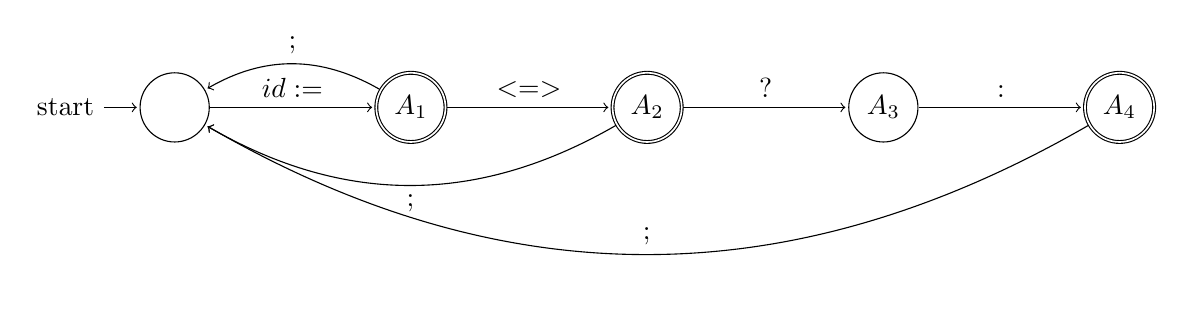
\begin{tikzpicture}[shorten >=1pt,node distance=3cm,on grid,auto]
	\node[state,initial] (q0) {};
	\node[state,accepting] (q1) [right of=q0] {$A_1$};
	\node[state,accepting] (q2) [right of=q1] {$A_2$};
	\node[state] (q3) [right of=q2] {$A_3$};
	\node[state,accepting] (q4) [right of=q3] {$A_4$};
	\path[->]
	(q0) edge node {$id:=$} (q1)
	(q1) edge node {$<=>$} (q2)
		 edge [bend right] node [above]{$;$} (q0)
	(q2) edge node {$?$} (q3)
		 edge [bend left] node {$;$} (q0)
	(q3)

		 edge node {$:$} (q4)
	(q4) edge [bend left] node [above]{$;$} (q0)
	;
\end{tikzpicture}


\includepdf[pages={1}]{figs/TheGrammar.pdf}
\end{document}